% Following the previous findings, this chapter will research and implement a Recurrent Neural Network using voltage, current, temperature and the known state of a battery charge to predict and feed forward the outputted result.
% It meant to use methodology constructed from the previous chapter:
% \begin{itemize}
%     \item Use single-cell data over the entire temperature range for a single profile, use FUDS for better performance capture.
%     \item Train a model with recommended modifications.
%     \item Verify the model against another cell with the same profile.
%     \item Validate the performance against the other two profiles, DST and US06.
% \end{itemize}

%
%
%There have been several attempts to determine the most effective strategy for model training.
%Both LSTM and Gradient Recurrent Unit are effective, and there is no noticeable difference in the impact between speed and outputted accuracy.
The previous chapter has analysed and discussed multiple implementations of RNN models to determine the State of Charge from sensory data like Voltage, Current and Temperature.
The research results have concluded that sensory data in one driving behaviour effectively predicts that specific driving behaviour but is poor at extrapolating to others by doubled error at best.
Thus, the battery state became a matter of not the battery itself but the accuracy and usage of the measurements.
Besides, the internal resistance of batteries creates voltage drops during the current drain.
The ability to accommodate such loss and still keep track of the State of Charge defines the quality of the ML model.
A potential solution to the problem is integrating SoC as one of the input features of a NN model.
The limitation here is to get the State of Charge in real-time.
There are two approaches to this: Charge estimation from other means, CC or three feature-based NN methods, or the Feed-Forward method to propagate the output value of the charge as an input into the next prediction.

%
%
The correction of the limitations identified in Chapter~\ref{cha:Analysis}, such as a training cross-accurate model and minimisation of resistance influence, will require implementing a new 4-feature-based method.
In this chapter, the Long short-term memory model will be developed, with a history of approximately 8 minutes and 20 seconds usage (500 samples at 1Hz), to predict the current State of Charge and propagate the result further into the next prediction.
Furthermore, a novel method of the training loop model will be proposed to eliminate the possibility of accumulating errors and the charge value.
It utilises the Autoregressive technique to introduce an adaptive and robust solution to training with some training output inaccuracy over time.
Furthermore, it forces the model to consider the potential of having variations in the State of Charge history and not fail the prediction in the following outputs.

%
%
% The rest of this paper is organised as follows: a methodology for an RNN model discussed in Section 2.
% The details of how auto-regression has been utilised are in Section 3.
% Subsections 4.1 and 4.2 separate points of model validation and process of parameter estimation.
% Finally, section 5 concludes the research by outlining several observations, which may require separate consideration.
% Most were isolated to closed scenarios with provided data or from battery cycling machines.
% The most promising approach to improve a model and make it more universal is to increase complexity. While some introduced deeper layer networks, others added additional mechanisms to those already used.
\begin{landscape}
    \begin{figure}[ht]
        \centering
        % 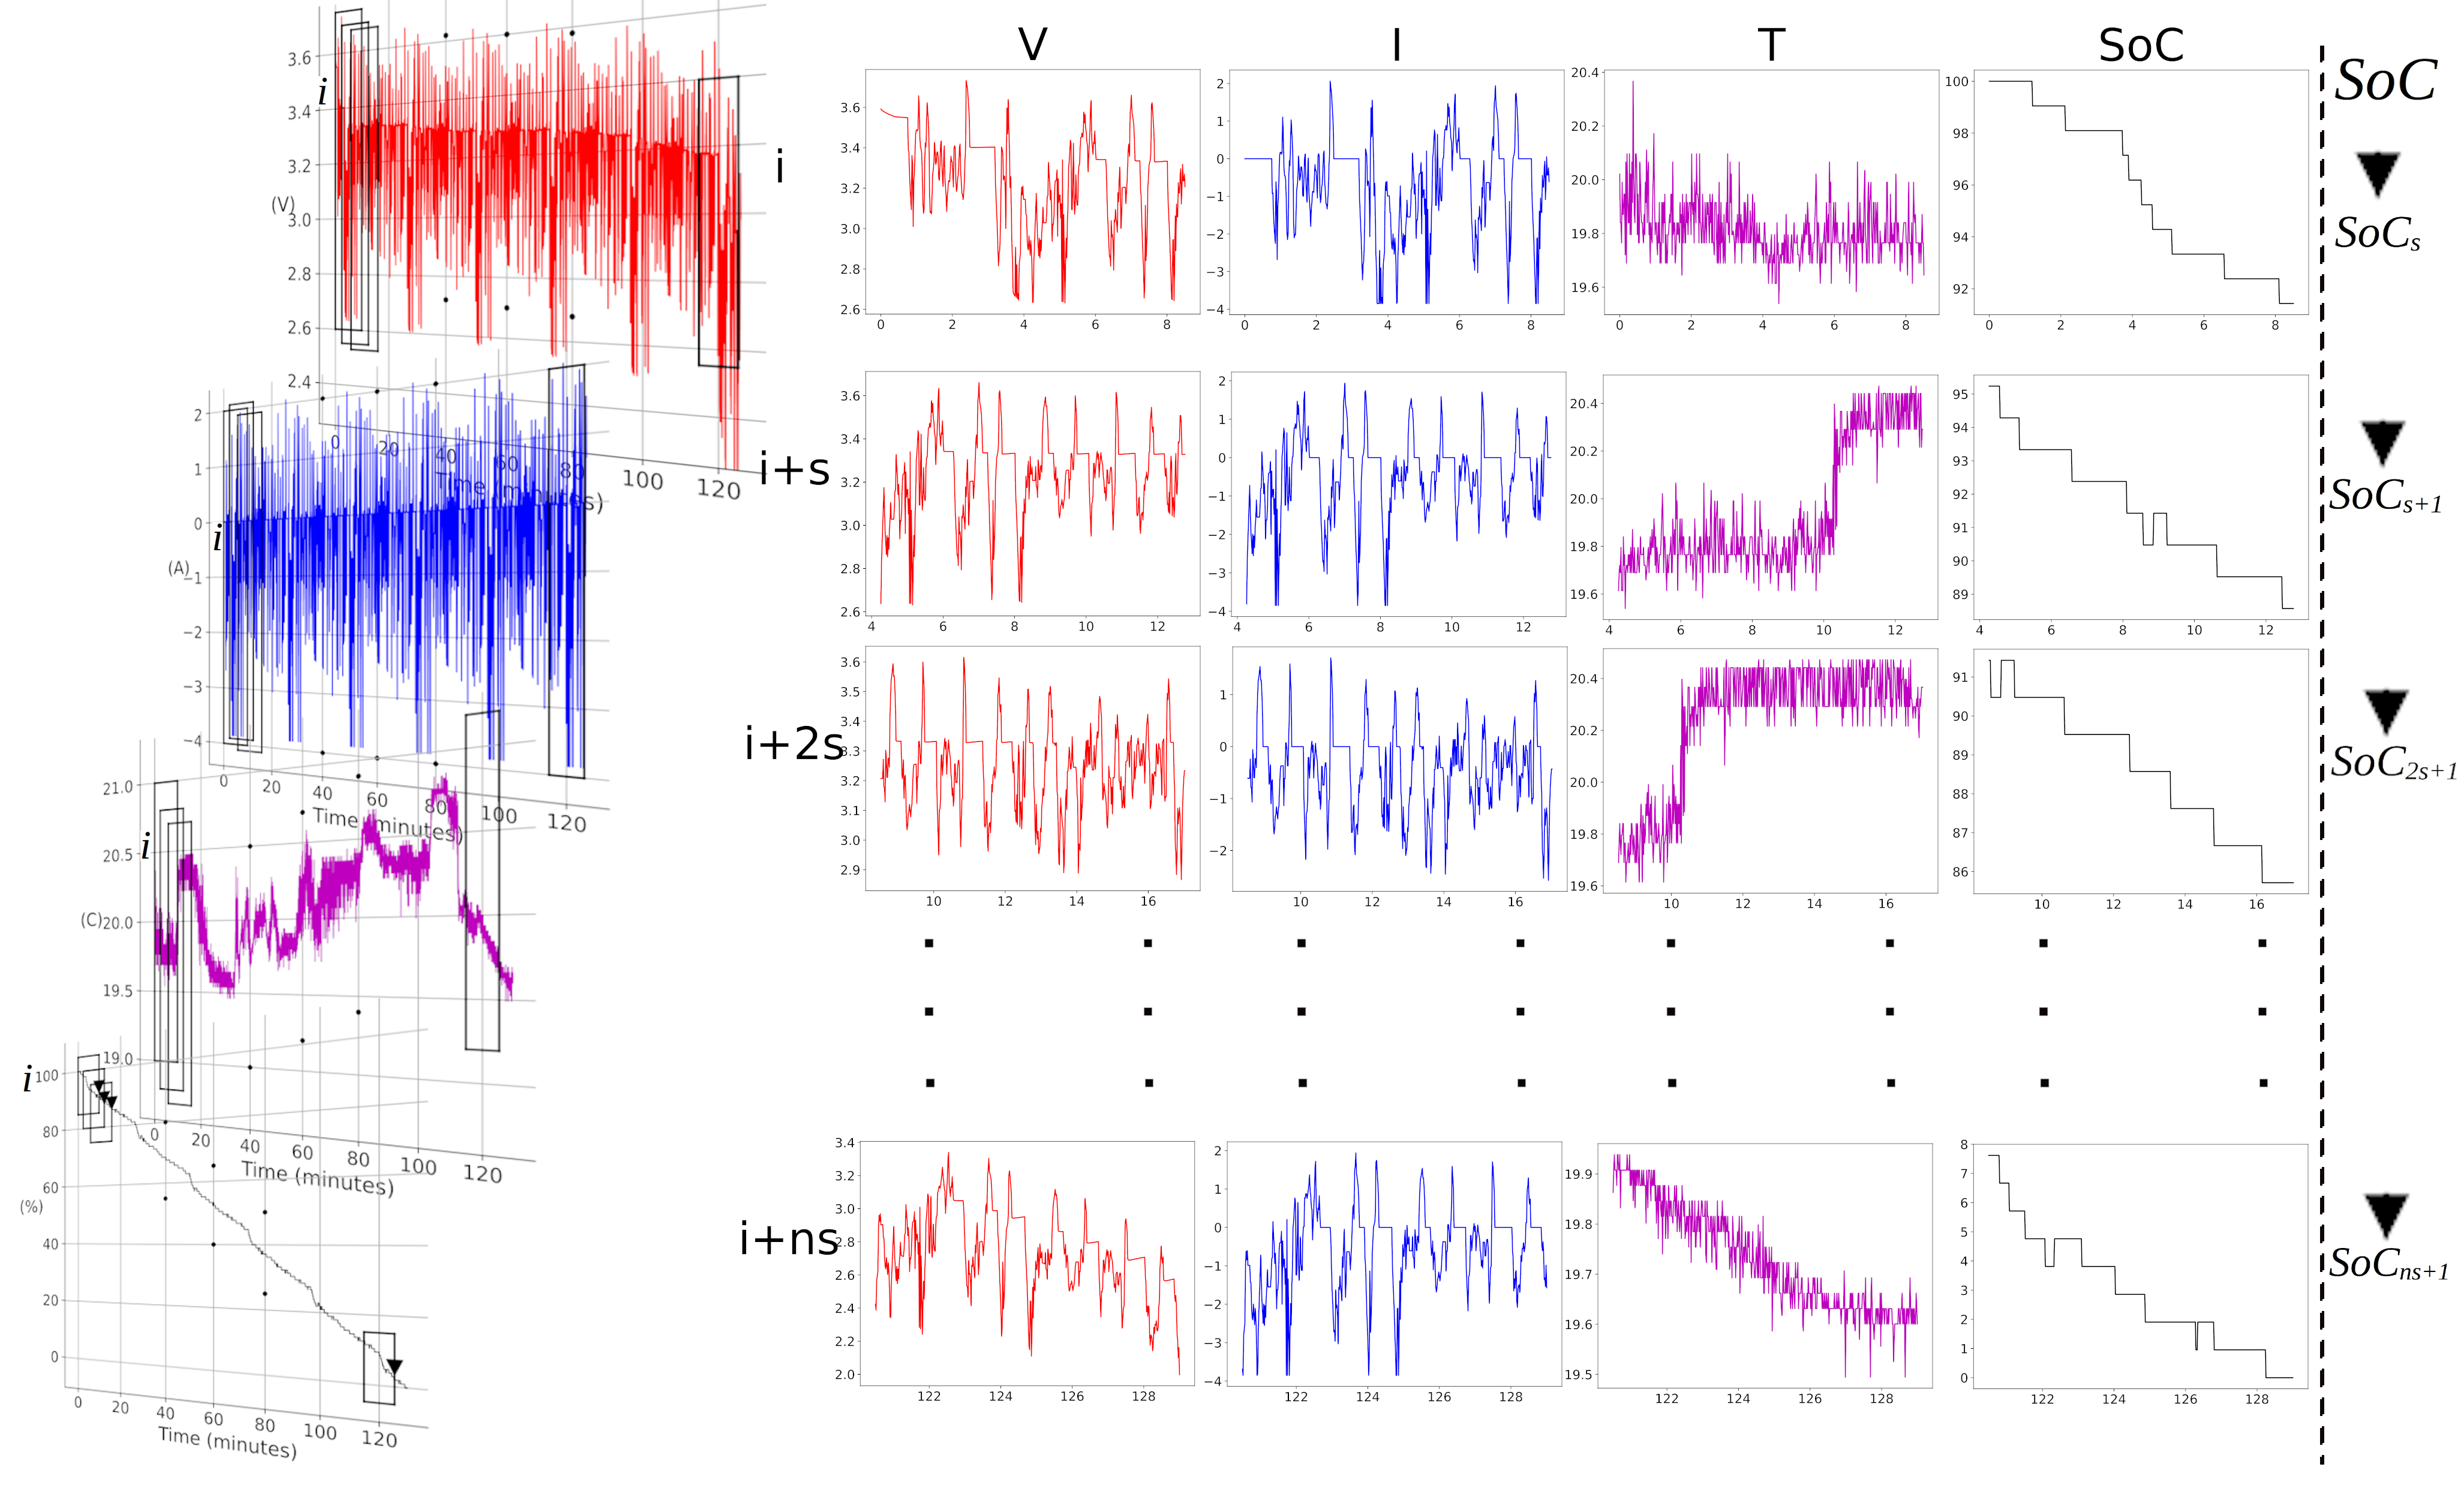
\includegraphics[width=0.9\linewidth]{II_Body/images/Windowing3D-1.jpg}
        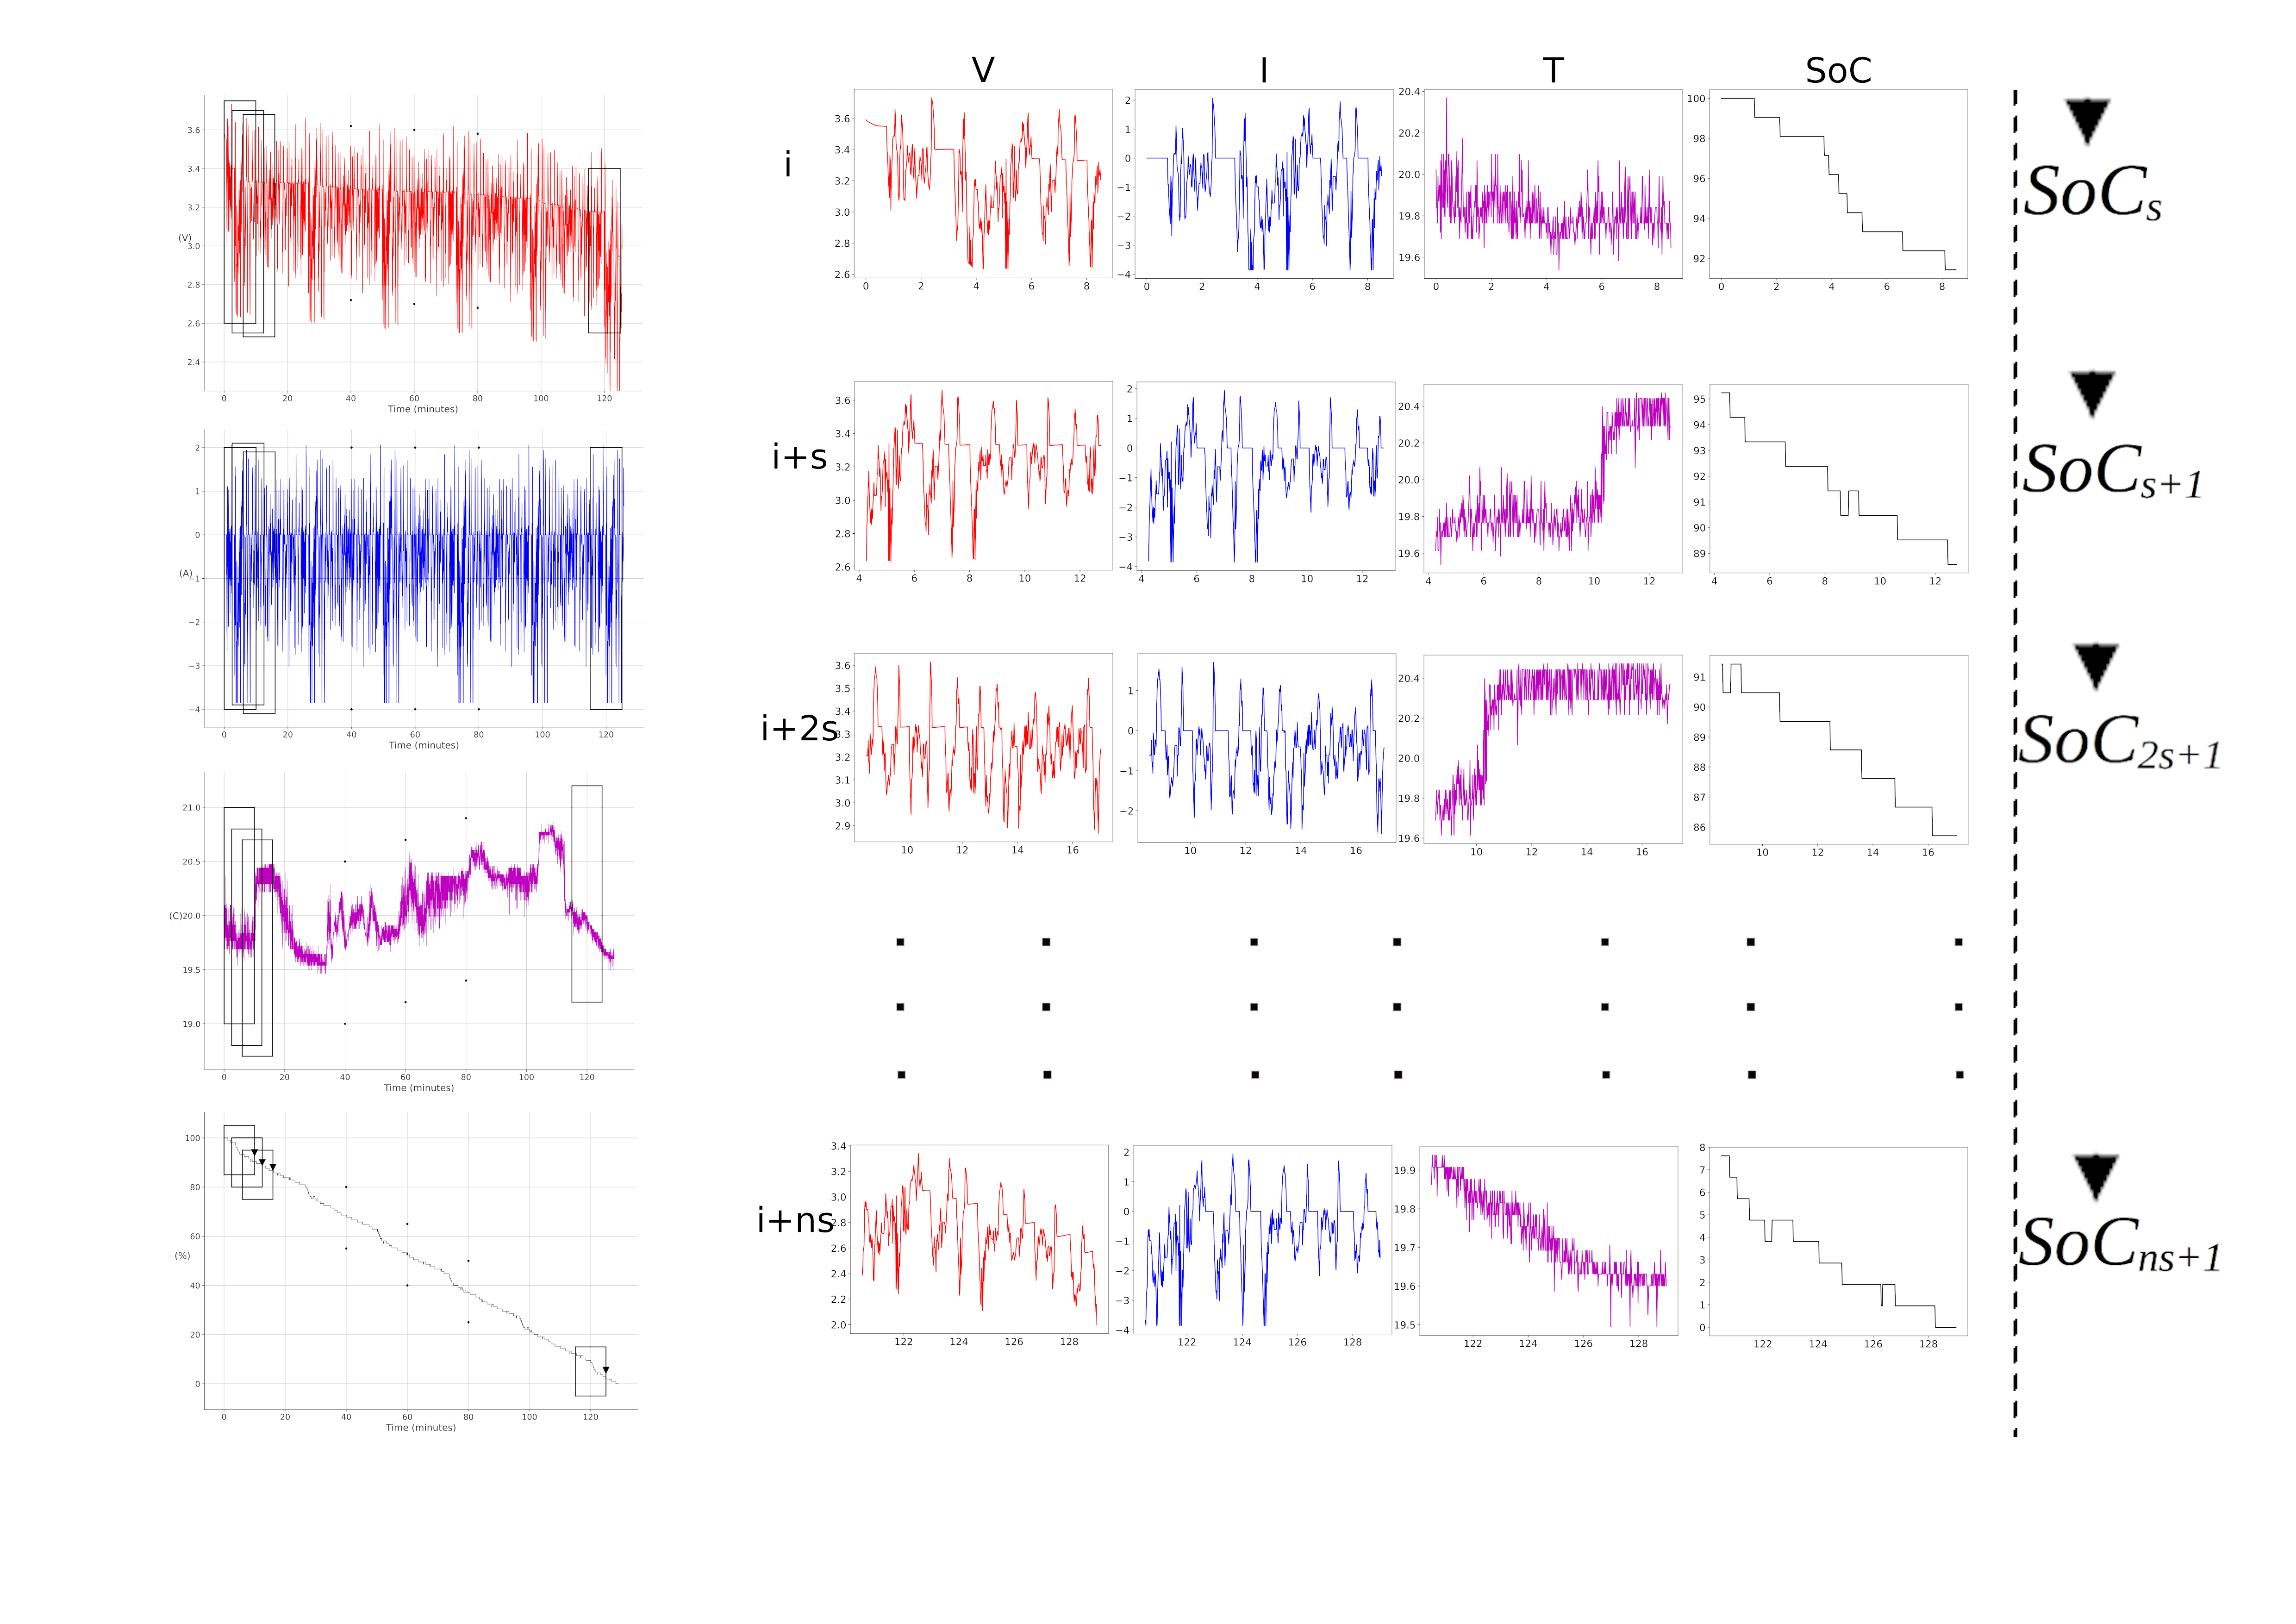
\includegraphics[width=0.9\linewidth]{II_Body/images/Windowing4f-A3.jpg}
        \caption{Data Windowing scheme at 1Hz sampling rate with four features and one output. For visualisation purposes, the $s$-step has been used as 250 seconds, which is different from the actual implementation. The initial index $i$ was kept as a value close to the beginning of the data, around zero.}
        \label{fig:Windowing}
    \end{figure}
\end{landscape}